\documentclass[compress]{beamer}
\usepackage{ifthen,verbatim,ulem,hyperref}

\newcommand{\isnote}{}
\xdefinecolor{lightyellow}{rgb}{1.,1.,0.25}
\xdefinecolor{darkblue}{rgb}{0.1,0.1,0.7}

%% Uncomment this to get annotations
%% \def\notes{\addtocounter{page}{-1}
%%            \renewcommand{\isnote}{*}
%% 	   \beamertemplateshadingbackground{lightyellow}{white}
%%            \begin{frame}
%%            \frametitle{Notes for the previous page (page \insertpagenumber)}
%%            \itemize}
%% \def\endnotes{\enditemize
%% 	      \end{frame}
%%               \beamertemplateshadingbackground{white}{white}
%%               \renewcommand{\isnote}{}}

%% Uncomment this to not get annotations
\def\notes{\comment}
\def\endnotes{\endcomment}

\setbeamertemplate{navigation symbols}{}
\setbeamertemplate{headline}{\mbox{ } \hfill
\begin{minipage}{5.5 cm}
\vspace{-0.75 cm} \small
\end{minipage} \hfill
\begin{minipage}{4.5 cm}
\vspace{-0.75 cm} \small
\begin{flushright}
\ifthenelse{\equal{\insertpagenumber}{1}}{}{Jim Pivarski \hspace{0.2 cm} \insertpagenumber\isnote/\pageref{numpages}}
\end{flushright}
\end{minipage}\mbox{\hspace{0.2 cm}}\includegraphics[height=1 cm]{../cmslogo} \hspace{0.1 cm} \includegraphics[height=1 cm]{../tamulogo} \hspace{0.01 cm} \vspace{-1.05 cm}}

\begin{document}
\begin{frame}
\vfill
\begin{center}
\textcolor{darkblue}{\Large Alignment of the DT chambers}

\vfill
\begin{columns}
\column{0.3\linewidth}
\begin{center}
\large
\textcolor{darkblue}{Jim Pivarski}

\vspace{0.2 cm}
Alexei Safonov
\end{center}
\end{columns}

\begin{columns}
\column{0.3\linewidth}
\begin{center}
\scriptsize
{\it Texas A\&M University}
\end{center}
\end{columns}

\vfill
29 January, 2009

\end{center}
\end{frame}

%% \begin{notes}
%% \item This is the annotated version of my talk.
%% \item If you want the version that I am presenting, download the one
%% labeled ``slides'' on Indico (or just ignore these yellow pages).
%% \item The annotated version is provided for extra detail and a written
%% record of comments that I intend to make orally.
%% \item Yellow notes refer to the content on the {\it previous} page.
%% \item All other slides are identical for the two versions.
%% \end{notes}

\small

\begin{frame}
\frametitle{Summary}
\begin{itemize}
\item We present alignment constants for the DT chambers, reducing
  misalignment from the 5--10~mm level down to the 1--2~mm level
\begin{itemize}
\item links DT chambers to the tracker's coordinate system using globalMuons
\item compatible with the latest tracker description (geometry, APEs,
  Lorentz-angle), TIB and TOB only (best-aligned part)
\item this is an update to the CRAFT\_ALL\_V4 muon geometry
  description, updating only those chambers with adequate statistics,
  keeping previously-aligned layer and superlayer substructure
\end{itemize}

\item Understanding of systematic effects
\begin{itemize}
\item control of errors from $\vec{B}$-field mismodelling
\item for other systematic effects, see DT-DPG presentation

\textcolor{blue}{\tt \scriptsize \href{http://indico.cern.ch/conferenceDisplay.py?confId=51267}{http://indico.cern.ch/conferenceDisplay.py?confId=51267}}
\end{itemize}

\item Validation plots: see DT-DPG ``more information'' for \mbox{every chamber\hspace{-1 cm}}
\begin{itemize}
\item a few examples shown here
\end{itemize}
\end{itemize}
\end{frame}

\begin{frame}
\frametitle{Basic algorithm (very quickly)}

\begin{enumerate}
\item Refit globalMuon tracks with zero weight on the muon hits, so that the tracks are determined entirely by the tracker, yet contain muon hits
\begin{itemize}
\item automatically in tracker's coordinate system
\item no coupling between track-fitting and alignment: convergence in one iteration (two performed)
\end{itemize}

\item Find the peak of the residuals distribution, note offset from zero
\begin{itemize}
\item weighted-average 1-D hits in the same chamber on the same track, to properly account for their correlation
\end{itemize}

\item Apply corrections to move residuals to zero
\begin{itemize}
\item DT local $x$ (global $r\phi$) coordinate: offset of local $x$ residuals
\item DT local $y$ (global $z$) coordinate: offset of local $y$ residuals
\item DT local $\phi_z$ (rotation in layer's plane): slope in local $x$ versus local $y$
\end{itemize}

\item Follow-up with detailed validation plots
\end{enumerate}
\end{frame}

\begin{frame}
\frametitle{Effect of $\vec{B}$-field mismodelling}

\begin{itemize}
\item Magnetic field is not properly described in reconstruction
\item Track propagation is sensitive to integral of $\vec{B}$-field error along \mbox{its path\hspace{-1 cm}}
\item How can we get reliable residuals?
\end{itemize}

\begin{columns}
\column{0.6\linewidth}
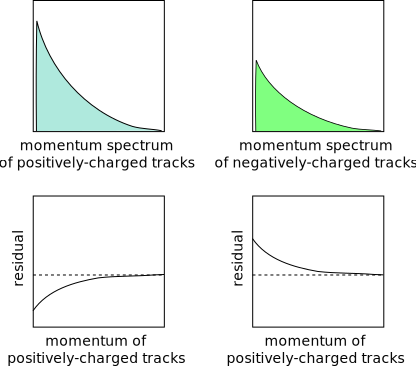
\includegraphics[width=\linewidth]{momentum_explanation.png}

\column{0.4\linewidth}
\vspace{-1 cm}
\begin{itemize}
\item Number of positively-charged and negatively-charged muons is not
  equal, but the momentum spectra are identical (fact used in charge
  ratio analysis)

\item Small deviations of reconstructed track from average muon
  trajectory is antisymmetric with charge
\end{itemize}
\end{columns}
\end{frame}

\begin{frame}
\frametitle{Effect of $\vec{B}$-field mismodelling}

\vspace{0.5 cm}
\begin{columns}
\column{0.6\linewidth}
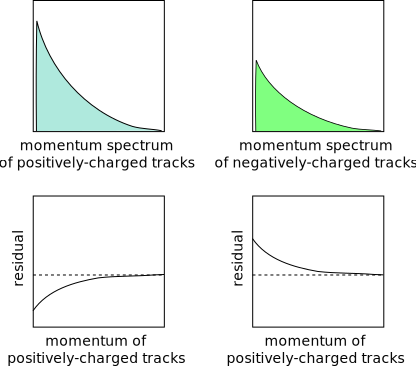
\includegraphics[width=\linewidth]{momentum_explanation.png}

\column{0.4\linewidth}
\vspace{-1 cm}
\begin{itemize}
\item Measure residuals peak in two bins, one for each charge
\item Non-weighted average is insensitive to $\vec{B}$-field errors

$\displaystyle \mbox{alignment} = \frac{R_+ + R_-}{2}$

\item Difference is maximally sensitive

$\displaystyle \mbox{error tracer} = \frac{R_+ - R_-}{2}$

\end{itemize}
\end{columns}

\begin{itemize}
\item Effectively scales up negatively-charged muon statistics such that the two curves cancel
\item \mbox{$\displaystyle \mbox{Systematic error} = \left(\mbox{error tracer}\right) \times \left(\mbox{charge mismeasurement}\right) \times \frac{0.3}{2.3}$}

\textcolor{white}{$\mbox{Systematic error}$} $\sim \left(\mbox{error tracer}\right) \times \left(\mbox{a few percent or less}\right)$

\end{itemize}
\end{frame}

\begin{frame}
\frametitle{Effect of $\vec{B}$-field mismodelling}
\begin{itemize}
\item Demonstration in station 4 (largest $\vec{B}$-field errors):
\begin{itemize}
\item despite large $(R_+ - R_-)/2$ difference (``error tracer''),

\vspace{0.2 cm}
the $(R_+ + R_-)/2$ average cleanly breaks at chamber boundaries
\end{itemize}
\end{itemize}

\includegraphics[height=\linewidth, angle=90]{demo_of_bfield.pdf}

\scriptsize grey background is the raw 2-D residuals distribution

linear fits are only a guide for the eye: not used in alignment!
\end{frame}

%% \begin{frame}
%% \frametitle{Effect of multiple scattering}

%% \begin{itemize}
%% \item Alignment correction is the peak of the \mbox{residuals distribution because\hspace{-1 cm}}
%% \begin{itemize}
%% \item good tracks agree on the alignment correction
%% \item bad tracks ``disagree in their own special way''
%% \end{itemize}
%% \end{itemize}

%% \begin{columns}
%% \column{0.65\linewidth}
%% Scattering processes have long power-law tails, while
%%   central resolution is Gaussian. \mbox{Fit function:\hspace{-1 cm}}

%% \vspace{-0.5 cm}
%% \begin{multline*}
%% f(x) = \int_{-\infty}^\infty \frac{1}{\pi}\frac{\Gamma/2}{(x - \xi)^2 + (\Gamma/2)^2} \times \\
%% \frac{1}{\sqrt{2\pi} \sigma} \exp\left(\frac{-\xi^2}{2 \sigma^2}\right) \, d\xi
%% \end{multline*}

%% The peak of every subset of residuals is determined from an unbinned fit

%% \column{0.35\linewidth}
%% \includegraphics[width=\linewidth]{fitfunction.pdf}
%% \end{columns}

%% \begin{itemize}
%% \item regular mean ($\sum x_i/N$) is mathematically \\ equal to the center of an unbinned Gaussian fit
%% \item this is a small generalization: only added tails
%% \item tails de-emphasize outliers because power-law contributes far less to log likelihood than exponential
%% \end{itemize}
%% \end{frame}

\begin{frame}
\frametitle{Track-based validation}

\begin{itemize}
\item Plot residuals with more detail than the alignable level
\begin{itemize}
\item dataset is divided such that you're only ever looking at one chamber at a time
\item grey background is the raw 2-D residuals distribution
\item linear fits are only a guide for the eye, not used in alignment
\item example of unaligned chamber: wheel~$-$2, station~2, sector~11
\item see DT-DPG Indico page ``more information'' for 152 pages
\end{itemize}
\end{itemize}

\vspace{-0.4 cm}
\begin{center}
\includegraphics[height=0.95\linewidth, angle=90]{summary_DTrphiVsZ_st2_sr11.pdf}
\end{center}
\end{frame}

\begin{frame}
\frametitle{Summary of residuals}

\begin{itemize}
\item To summarize, project all residuals ($p_T > 80$~GeV, all chambers)
\begin{itemize}
\item like the tracker's $\chi^2/N_{\mbox{\scriptsize dof}}$ plot, but unweighted
\item less sensitive measure of alignment, but convenient
\end{itemize}
\item Residuals in plots are calculated the same way as residuals \mbox{in alignment\hspace{-1 cm}}
\end{itemize}

\begin{columns}
\column{0.25\linewidth}
\includegraphics[width=\linewidth]{raw_station1.pdf}

\includegraphics[width=\linewidth]{rawz_station1.pdf}

\column{0.25\linewidth}
\includegraphics[width=\linewidth]{raw_station2.pdf}

\includegraphics[width=\linewidth]{rawz_station2.pdf}

\column{0.25\linewidth}
\includegraphics[width=\linewidth]{raw_station3.pdf}

\includegraphics[width=\linewidth]{rawz_station3.pdf}

\column{0.25\linewidth}
\includegraphics[width=\linewidth]{raw_station4.pdf}
\end{columns}
\end{frame}

\begin{frame}
\frametitle{Linearly-independent validation}

\begin{itemize}
\item Linearly-independent test: residuals differences between
  \mbox{pairs of stations\hspace{-1 cm}}

\mbox{$\mbox{difference} = \big(\mbox{st.\ 3 track} - \mbox{st.\ 3 hit}\big) - \big(\mbox{st.\ 2 track} - \mbox{st.\ 2 hit}\big)$}

\begin{itemize}\setlength{\itemsep}{0.1 cm}
\item shows {\it relative} positions of chambers; globalMuon is just a ruler
\item therefore, this is a real consistency check
\item note zoomed vertical scale: accuracy is 1--2~mm
\item also shows $\vec{B}$-field error between the stations, not integrated
\end{itemize}
\end{itemize}

\vspace{-0.4 cm}
\begin{center}
\includegraphics[height=0.95\linewidth, angle=90]{summary_DTrphidiff23VsPhi_whC.pdf}
\end{center}
\end{frame}

\begin{frame}
\frametitle{Values of the corrections}

\begin{columns}
\column{0.35\linewidth}
\includegraphics[width=\linewidth]{corrections_x.pdf}

\column{0.35\linewidth}
\includegraphics[width=\linewidth]{corrections_y.pdf}

\column{0.35\linewidth}
\includegraphics[width=\linewidth]{corrections_phiz.pdf}
\end{columns}

\vfill
\begin{itemize}
\item 5--10~mm changes in $r\phi$ positions, and they don't correspond to an overall rotation of the wheels

\item A scan of residuals differences plots suggests that remaining misalignment is on the order of 1--2~mm
\end{itemize}
\end{frame}

%% \section*{First section}
%% \begin{frame}
%% \begin{center}
%% \Huge \textcolor{blue}{First section}
%% \end{center}
%% \end{frame}

\begin{frame}
\frametitle{Constants in database}

\begin{itemize}
\item Constants were successfully uploaded to the database, but an
  additional 2~mm $\times$ wheel number was applied to the $z$
  positions
\begin{itemize}
\item track residuals do not prefer this additional translation
\item but $z$ residuals still have other effects on the same order, so
  the resolution is about 2~mm anyway
\item see Muon Alignment Hypernews for full SQLite-DB comparison
\end{itemize}
\end{itemize}

\vspace{-0.4 cm}
\begin{center}
\includegraphics[height=\linewidth, angle=90]{summary_DTzVsZ_st1_sr04.pdf}
\end{center}
\end{frame}

\begin{frame}
\frametitle{Conclusions}
\begin{itemize}\setlength{\itemsep}{0.25 cm}
\item New DT chamber alignment, in the same coordinate system as the tracker, reduces misalignment from the 5--10~mm level down to the 1--2~mm level
\item Covers mostly wheels $-$1, 0, and $+$1 (wherever statistics was sufficient)
\item Controls for systematics, not a blind minimization of residuals
\begin{itemize}
\item see DT-DPG for more
\end{itemize}
\item Constants are in the database, but with an extra $z$ translation
  that worsens the average $z$ residual
\end{itemize}
\label{numpages}
\end{frame}

\end{document}
